\documentclass{article}

\usepackage{geometry}
\usepackage{makecell}
\usepackage{array}
\usepackage{multicol}
\usepackage{setspace}
\usepackage{changepage}
\usepackage{booktabs}
\usepackage{graphicx}
\usepackage{cprotect}
\usepackage{float}
\newcolumntype{?}{!{\vrule width 1pt}}
\newcommand{\paragraphlb}[1]{\paragraph{#1}\mbox{}\\}
\renewcommand\theadalign{tl}
\setstretch{1.10}
\setlength{\parindent}{0pt}

\geometry{top=12mm, left=1cm, right=2cm}
\title{\vspace{-1cm}Netzwerktechnologien Aufgabenblatt 5}
\author{Andreas Hofer}

\begin{document}
	\maketitle
	\section{TCP}
	\begin{figure}[H]
	\centering
	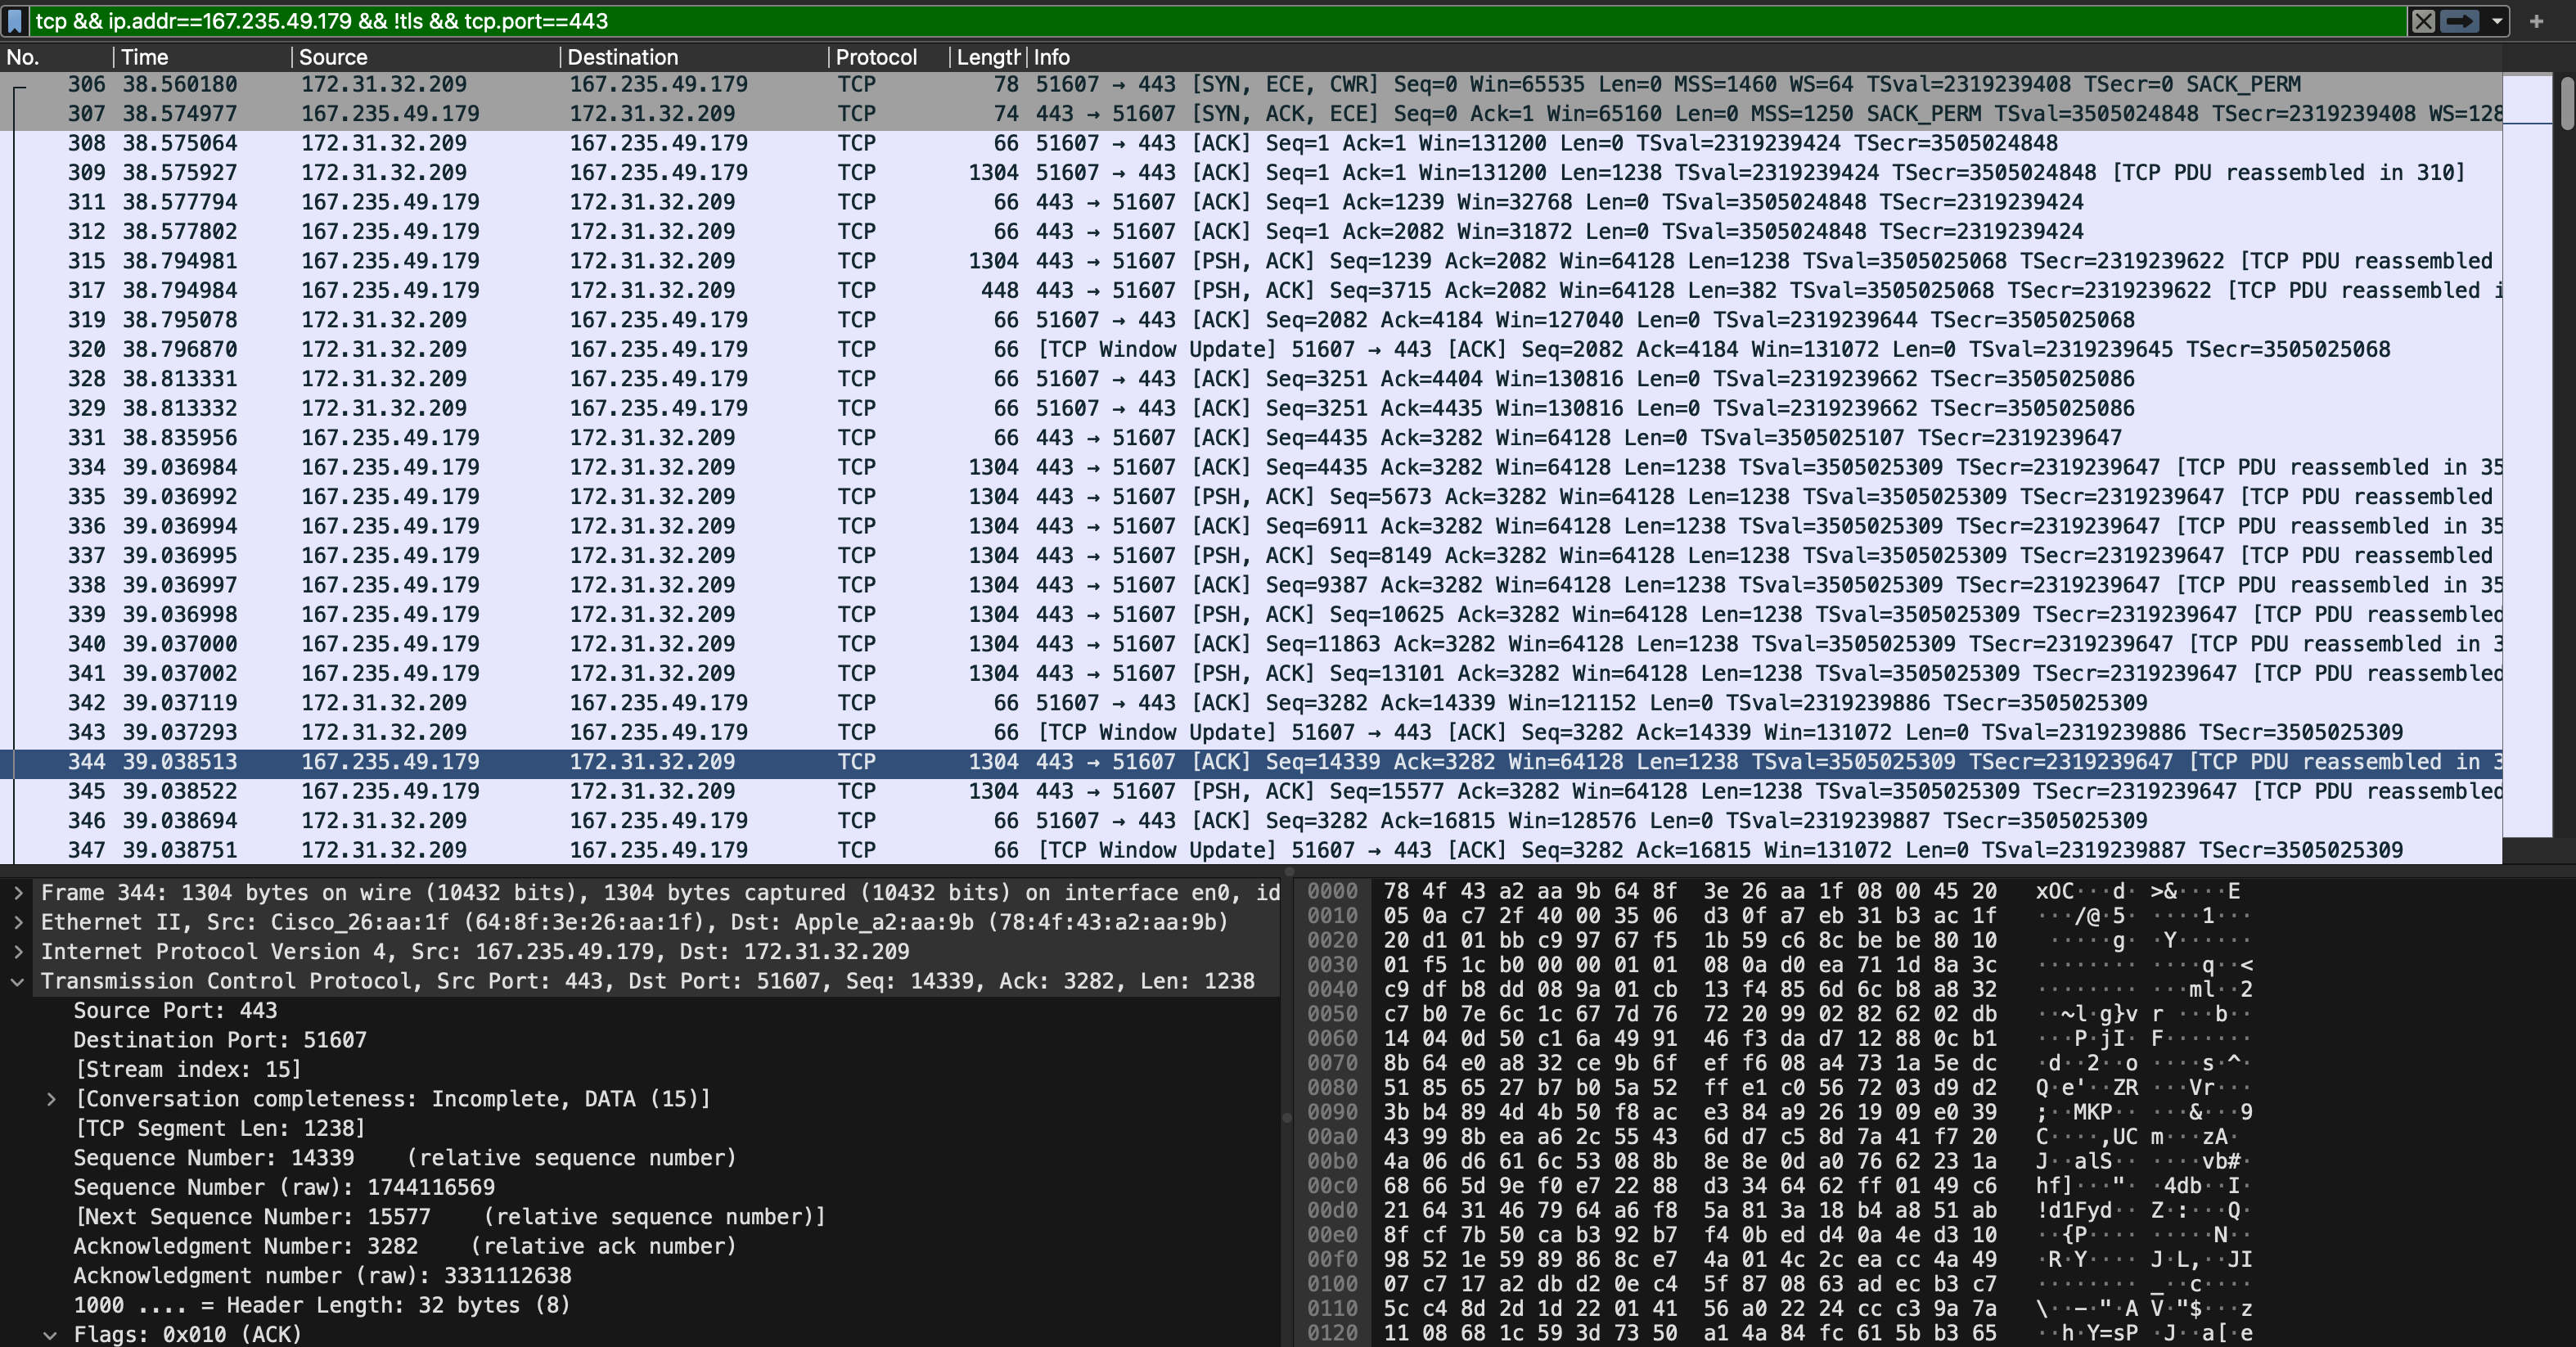
\includegraphics[scale=0.3]{Bilder/tcp.png}
	\caption{Die Wireshark Aufzeichnung des Websiteaufrufes}
	\end{figure}
	\addtocounter{subsection}{2}
	\subsection{Interpretation}
	Das erste was mir auffällt ist, dass \textit{sehr viele} Pakete verschickt werden. Knapp 500 in weniger als einer Sekunde, was Sinn macht, wenn man bedenkt, wie groß eine Website mit Bildern ist. Abgesehen davon ist die Funktionsweise von TCP gut erkennbar. Zuerst wird die Verbindung mit SYN aufgebaut, und danach werden die Pakete gesendet und die acknowledgements erhalten.
	\subsection{Retransmission}
	\begin{figure}[H]
	\centering
	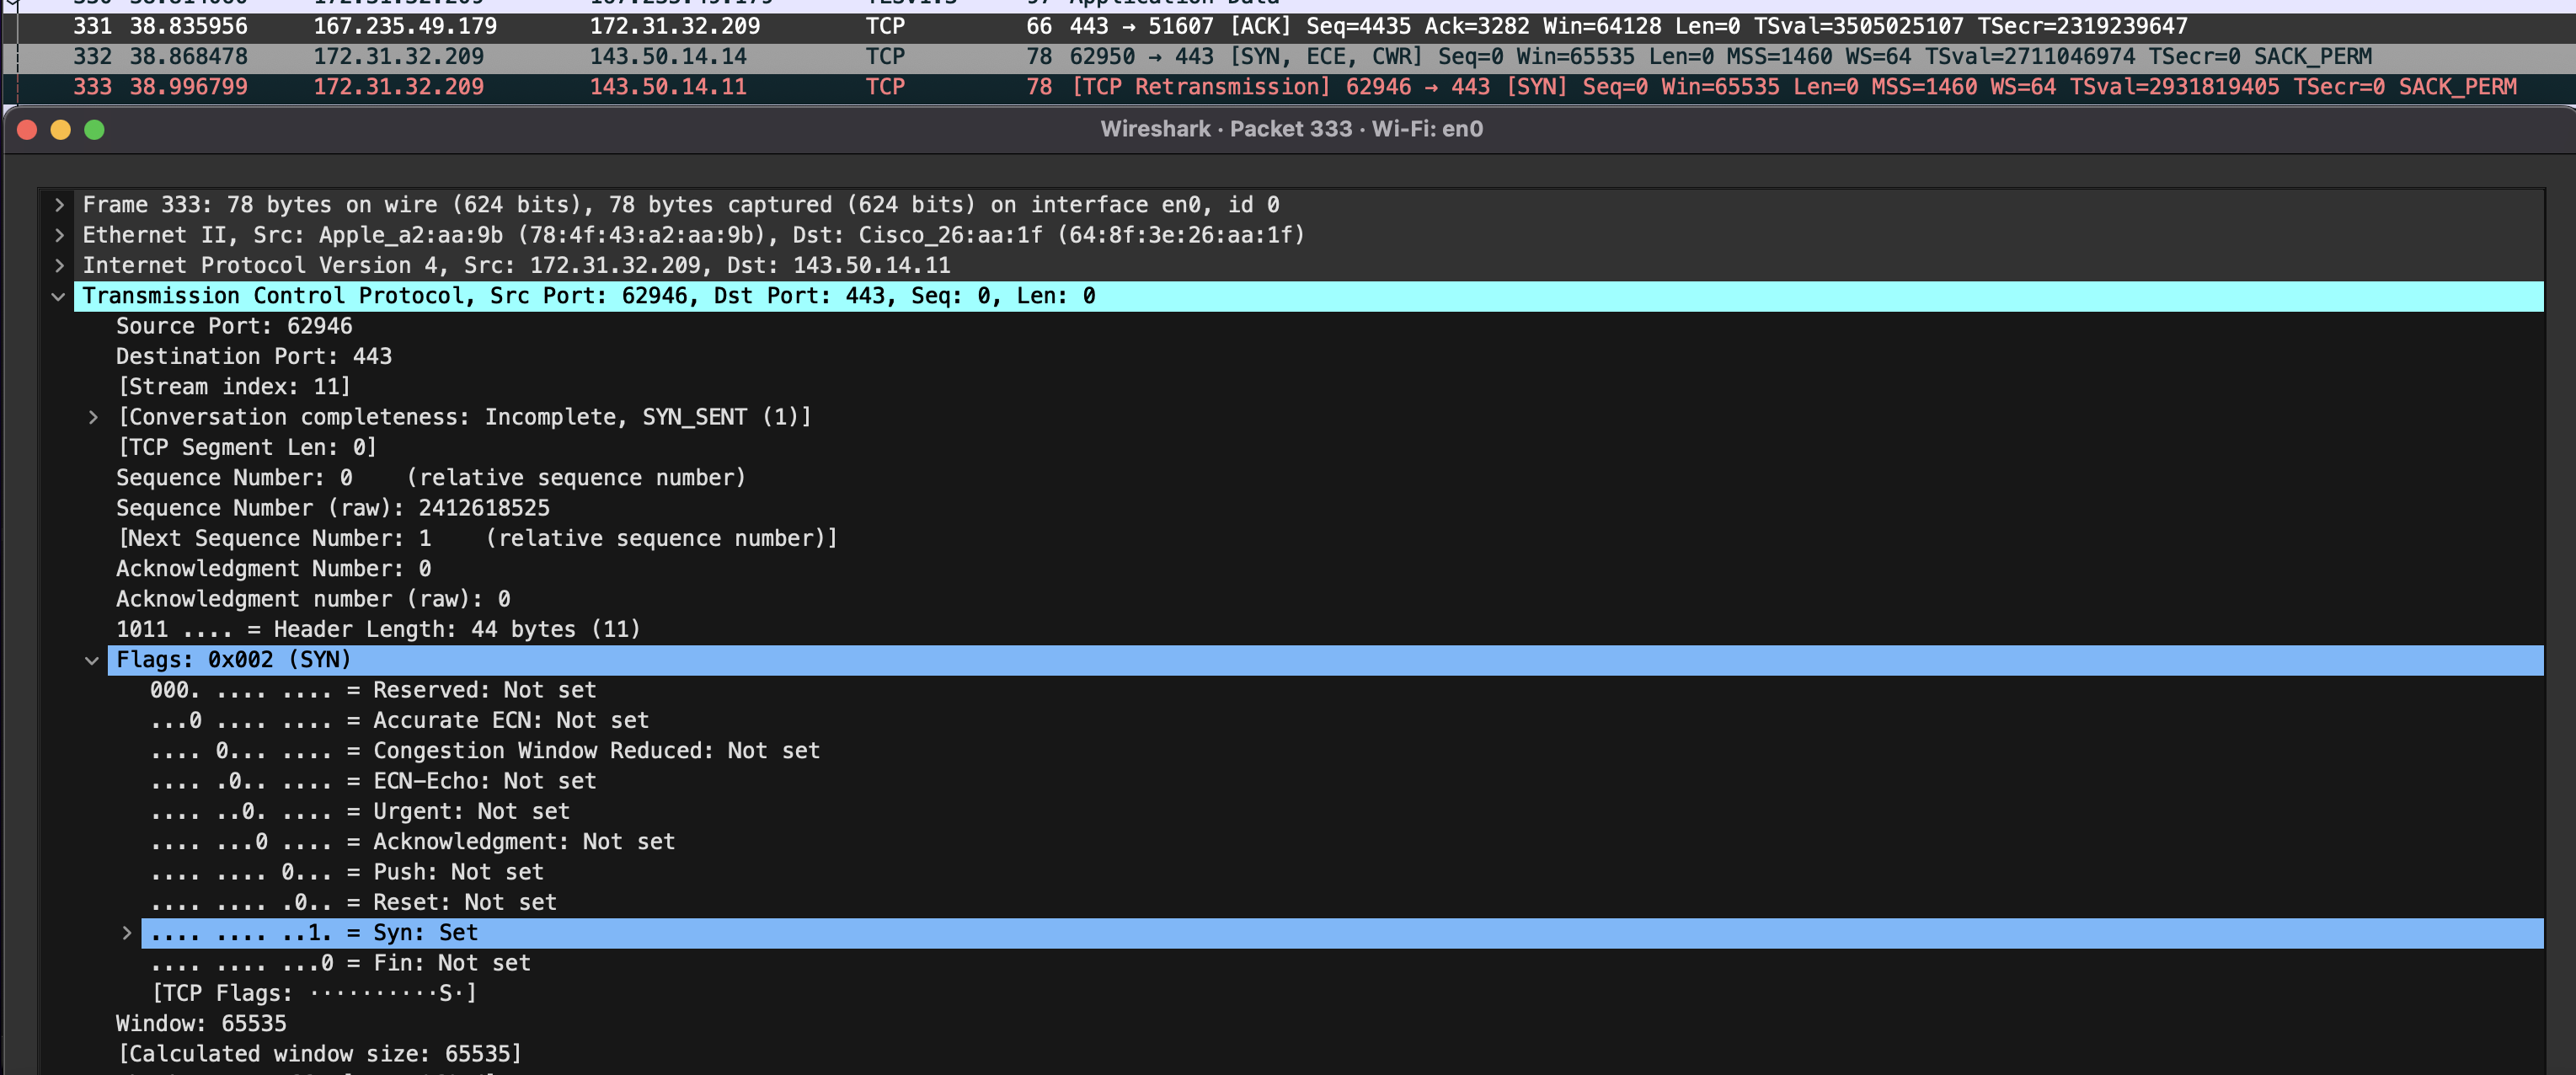
\includegraphics[scale=0.3]{Bilder/retransmission.png}
	\caption{Ein TCP Retransmission Paket und der Inhalt. Das Paket ist nicht ausgewählt damit man die Farbe sieht.}
	\end{figure}
	Die schwarz hinterlegten Pakete mit rotem Text, werden von Wireshark mit \verb|Retransmission| gekennzeichnet, also ist das höchstwahrscheinlich das erneute Senden eines TCP Pakets nachdem das acknowledgement nicht rechtzeitig zurückgekommen ist. Zu beachten ist auch die gesetzte SYN flag. Es scheint zum Glück nicht so als ob besonders viele Pakete verloren gehen.
	\section{DNS}
	\cprotect\subsection{\verb|nslookup|}
	\addtocounter{subsubsection}{3}
	\cprotect\subsubsection{\verb|nslookup|  Wiresharkaufzeichnung}
	\begin{figure}[H]
	\centering
	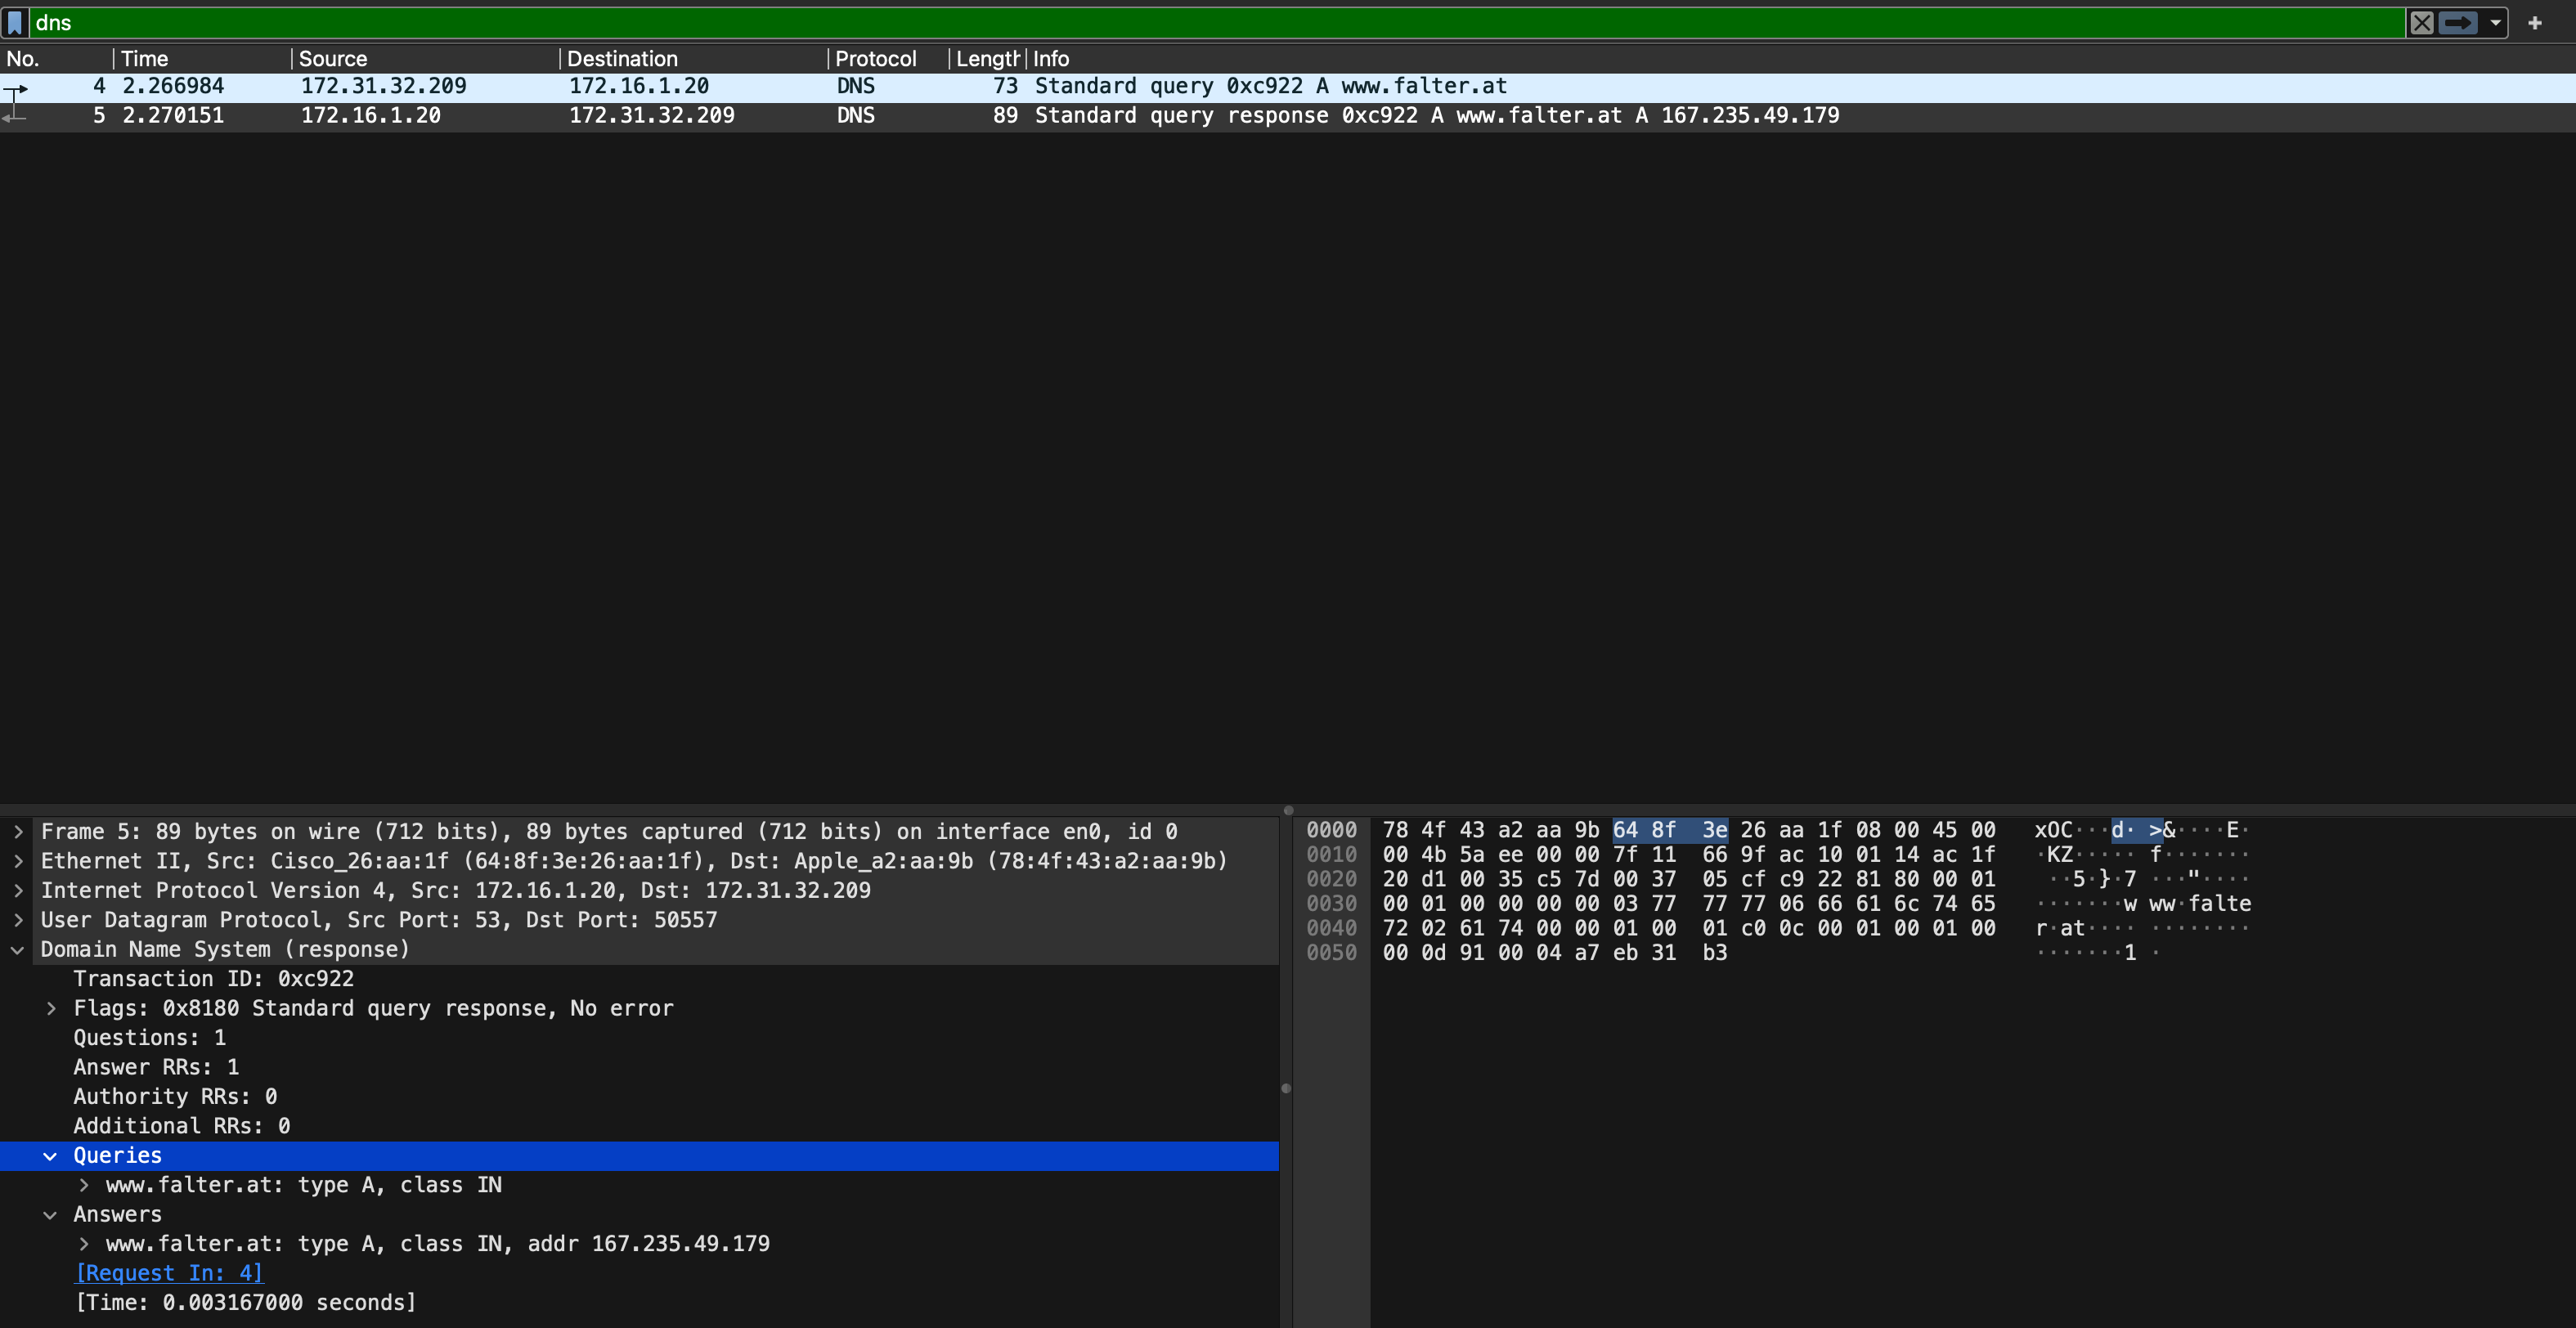
\includegraphics[scale=0.35]{Bilder/nslookup_ws.png}
	\cprotect\caption{Das aufgezeichnete DNS Paket von \verb|nslookup| }
	\end{figure}
	\cprotect\subsubsection{\verb|nslookup|  Command Line} 
	\begin{figure}[H]
	\centering
	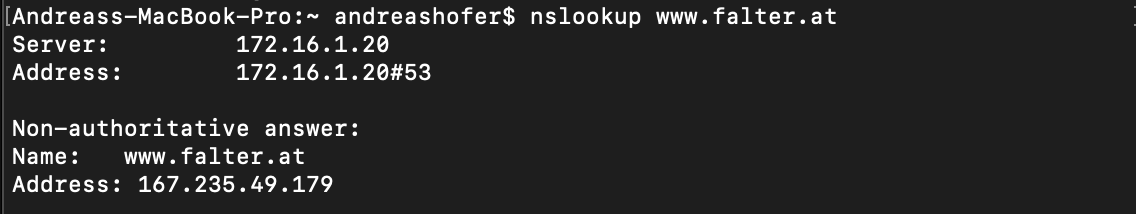
\includegraphics[scale=0.8]{Bilder/nslookup_cmd.png}
	\caption{Das Terminalfenster nach Ausführung des Befehls}
	\end{figure}
	\subsubsection{Interpretation}
	\verb|nslookup| scheint seinen output in zwei Teile anzugeben. Zuerst der DNS-Server von dem die Antwort gekommen ist (in diesem Fall \verb|172.16.1.20|) sowie dessen Netzwerk. Dann die Antwort selbst mit der Information ob die Info von einem Auritativen oder Nicht-Autoritativen Server gekommen ist (In diesem Fall war es wahrscheinlich der lokale DNS Server statt des DNS Servers der die \verb|.at| Adresse verwaltet.) 
	\cprotect\subsection{\verb|dig|}
	Leider funktionierte der \verb|dig +trace| Befehl in meinem Terminal nicht und gab immer nur einen Fehler zurück, weshalb ich die Webversion verwendet habe.
	\begin{figure}[H]
	\centering
	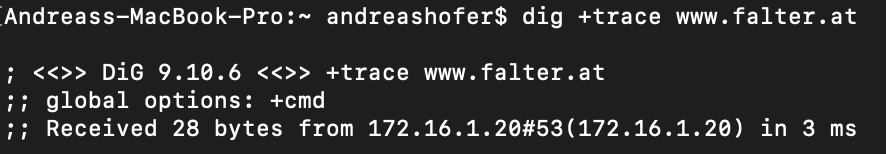
\includegraphics[scale=0.7]{Bilder/dig_cmd.png}
	\caption{Rückgabewert von dig in der command line. Das TCP Paket enthielt nur einen Fehler.}
	\end{figure}
	\begin{figure}[H]
	\centering
	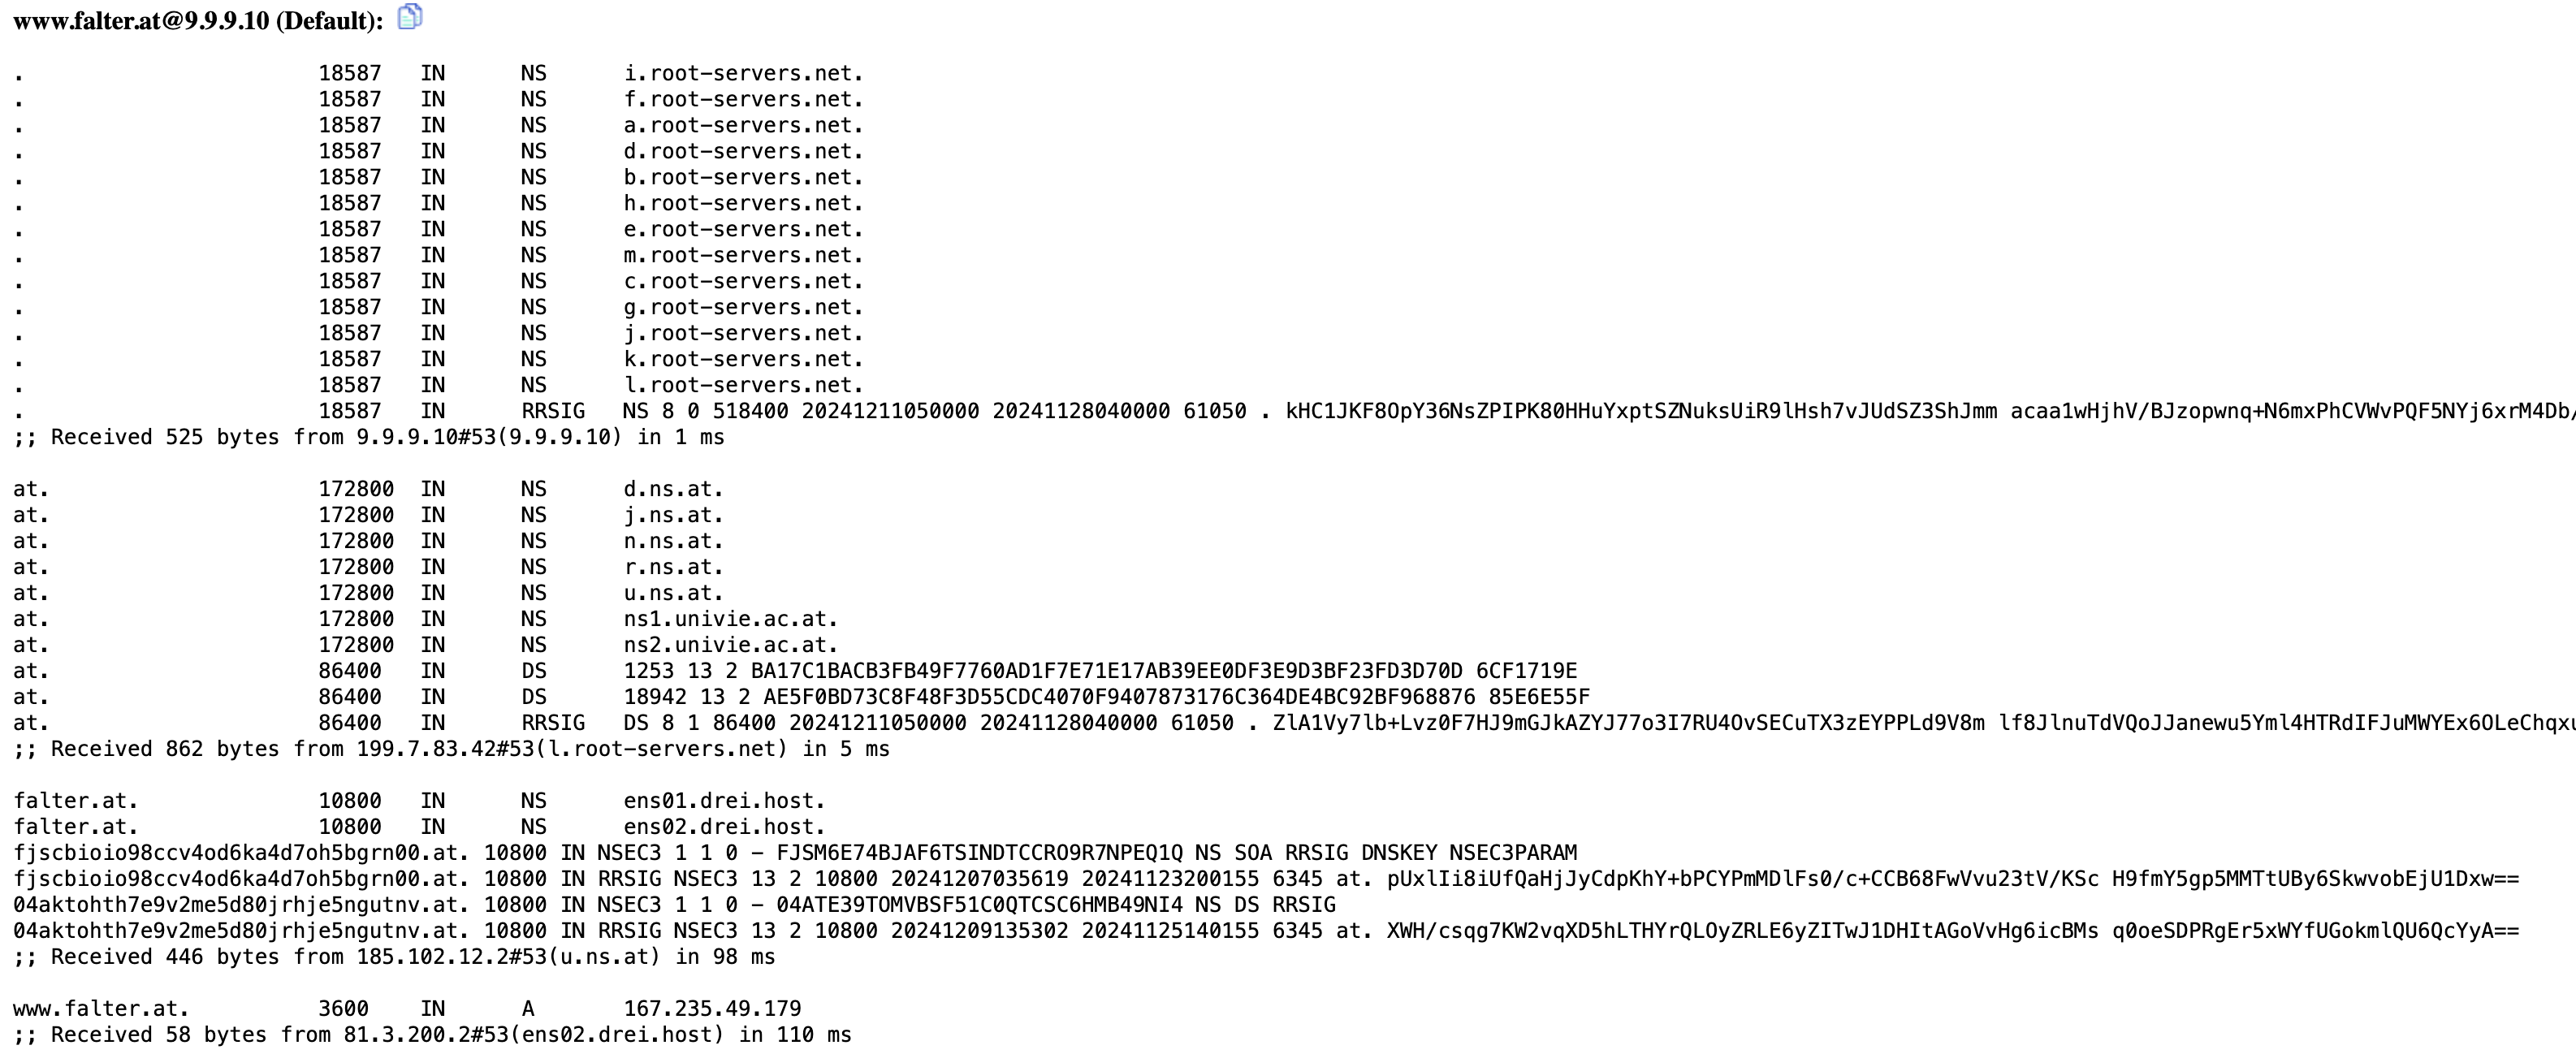
\includegraphics[scale=0.35]{Bilder/dig_web.png}
	\caption{\verb|dig| trace von digwebinterface.com }
	\end{figure}
	\verb|dig| funktioniert nach einem iterativen Prozess, indem es jeweils einen DNS Server nach der Webadresse fragt, diese Rückgabetabelle dann ausgibt und einen dieser Server nach der nächsten Tabelle befragt. So hat er zuerst \verb|9.9.9.10|, einen DNS Server von \verb|quad9|  befragt, dann den root-server \verb|l| unter \verb|199.7.83.42|, danach den name server \verb|u| unter \verb|185.102.12.2| und schließlich den name server von \verb|Drei| unter \verb|81.3.200.2| um zur IP Adresse \verb|167.235.49.179| zu gelangen.
	\cprotect\subsection{\verb|dig| vs \verb|nslookup|}     	
	\verb|nslookup| ist wesentlich älter als \verb|dig|, und hat auch einen kleineren Funktionsumfang. Obwohl  

	
	
	
	
\end{document}